\section{Pendahuluan}
\subsection{Latar Belakang}
Dalam dunia jaringan komputer, kemampuan untuk membangun koneksi fisik dan mengatur komunikasi antar perangkat sangat penting. Oleh karena itu, praktikum mengenai crimping dan routing IPv4 dilaksanakan sebagai upaya pembelajaran dasar dalam membangun infrastruktur jaringan. Crimping merupakan teknik penting dalam pembuatan kabel jaringan yang berfungsi untuk menghubungkan perangkat-perangkat jaringan secara fisik, sedangkan routing IPv4 digunakan untuk mengarahkan lalu lintas data antar jaringan berbeda menggunakan alamat IP versi 4. \\ Permasalahan yang sering muncul dalam implementasi jaringan komputer, seperti koneksi fisik yang tidak stabil akibat crimping yang salah, atau kegagalan komunikasi karena konfigurasi IP dan routing yang tidak tepat, menjadi alasan utama pentingnya praktikum ini dilakukan. Praktikum ini bertujuan untuk memberikan pemahaman praktis dalam menyusun kabel jaringan dengan standar yang benar, serta mengonfigurasi perangkat agar dapat saling berkomunikasi melalui protokol IPv4 secara efisien. \\ Penguasaan konsep dan praktik crimping serta routing IPv4 menjadi bekal penting bagi mahasiswa dalam menghadapi tantangan dunia kerja yang menuntut keterampilan teknis jaringan komputer.

\subsection{Dasar Teori}
Jaringan komputer adalah sistem yang memungkinkan dua atau lebih perangkat komputer untuk saling terhubung dan bertukar informasi. Agar komunikasi antar perangkat berjalan lancar, jaringan memerlukan aturan yang disebut protokol. Protokol jaringan merupakan standar yang menentukan bagaimana data dikirim, diterima, dan diproses oleh perangkat dalam jaringan. Setiap komputer yang terhubung ke jaringan harus mengikuti protokol ini agar dapat saling berkomunikasi secara efektif. \\ Jaringan komputer sendiri dapat diklasifikasikan menjadi beberapa jenis berdasarkan cakupan wilayahnya, seperti LAN (Local Area Network) untuk area lokal seperti rumah atau kantor, MAN (Metropolitan Area Network) untuk cakupan antar gedung atau kampus dalam satu kota, WAN (Wide Area Network) seperti internet yang mencakup wilayah sangat luas, PAN (Personal Area Network) adalah jaringan berskala sangat kecil, biasanya digunakan untuk menghubungkan perangkat pribadi dalam jarak dekat, dan CAN (Campus Area Network) adalah jaringan yang mencakup area kampus atau institusi yang terdiri dari beberapa bangunan, dan menghubungkan banyak LAN dalam satu lokasi fisik. \\ Agar perangkat dalam jaringan bisa saling berkomunikasi, masing-masing harus memiliki alamat IP (Internet Protocol Address) yang unik. Alamat IP berfungsi seperti alamat rumah bagi perangkat, sehingga data dapat dikirim ke tujuan yang benar. IPv4 (Internet Protocol version 4) adalah protokol alamat IP yang paling umum digunakan, yang menggunakan sistem pengalamatan 32-bit dalam bentuk empat okta desimal, misal 192.168.1.1 . Penggunaan IPv4 sangat penting dalam proses routing, yakni pengaturan jalur data antarjaringan, serta dalam pengelompokan jaringan dengan metode subnetting. \\ Selain konfigurasi logis, jaringan juga memerlukan koneksi fisik. Dalam jaringan LAN, kabel UTP (Unshielded Twisted Pair) sering digunakan sebagai media transmisi data. Untuk menyambungkan kabel ke perangkat jaringan, dilakukan proses crimping, yaitu menempelkan konektor RJ45 ke ujung kabel UTP menggunakan alat khusus. Crimping harus dilakukan sesuai standar pengkabelan seperti T568A atau T568B agar tidak terjadi kesalahan koneksi. \\ Setelah perangkat saling terhubung secara fisik, perlu dilakukan konfigurasi routing agar perangkat dalam jaringan berbeda dapat saling berkomunikasi. Routing adalah proses pemilihan jalur terbaik untuk pengiriman data dari satu jaringan ke jaringan lain. Routing dapat dilakukan secara statis, di mana administrator menentukan jalur secara manual, atau dinamis, di mana router secara otomatis menyesuaikan jalur berdasarkan protokol tertentu seperti RIP atau OSPF.

%===========================================================%
\section{Tugas Pendahuluan}
\begin{enumerate}
	\item a. Rentang IP dan prefix tiap departemen: \\ RnD : 192.168.0.0/25 (Usable: 192.168.0.1–126) \\ Produksi : 192.168.0.128/26 (Usable: 192.168.0.129–190) \\ Administrasi : 192.168.0.192/27 (Usable: 192.168.0.193–222) \\ Keuangan : 192.168.0.224/28 (Usable: 192.168.0.225–238) \\ \\ b. total subnet yg diperlukan : tiap departemen membutuhkan 1 subnet jadi total subnet adalah 4. Dan IP network untuk masing masing departemen : \\ Rnd : 192.168.0.0/25 \\ Produksi : 192.168.0.128/26 \\ Administrasi : 192.168.0.192/27 \\ Keuangan : 192.168.0.224/28
	\item topologi sederhana 1 router 4 subnet
	\begin{figure}[H]
		\centering
		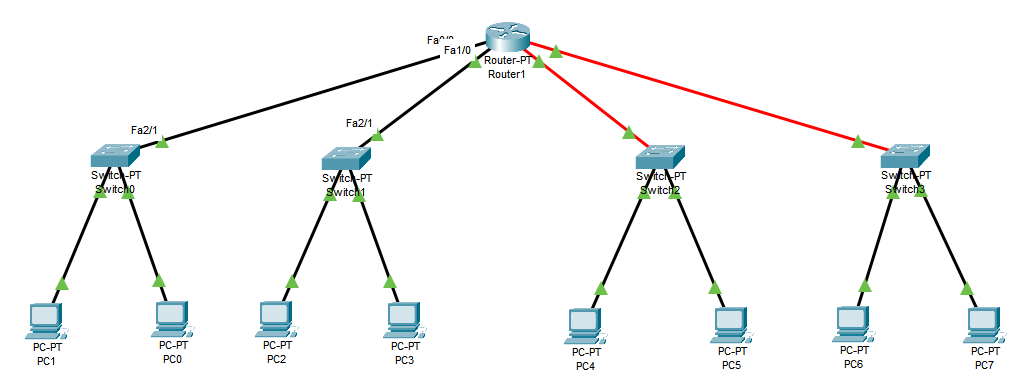
\includegraphics[width=0.65\linewidth]{image/Topologi sederhana.png}
		\label{fig:inirujukan}
	\end{figure}	
	\item tabel routing
	\begin{figure}[H]
		\centering
		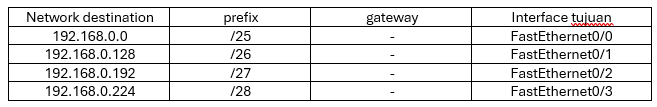
\includegraphics[width=0.8\linewidth]{image/tabel routing.png}
		\label{fig:inirujukan}
	\end{figure}
	\item Topologi sederhana ini cocok dengan static routing karena topologi yang kecil dan statis, tidak ada perubahan rute dinamis (banyak router bertukar informasi), mudah dikonfigurasi. 
\end{enumerate}